\subsubsection{UC - Gestione di prenotazioni per un utente scelto}

\begin{figure}[h]
  \centering
    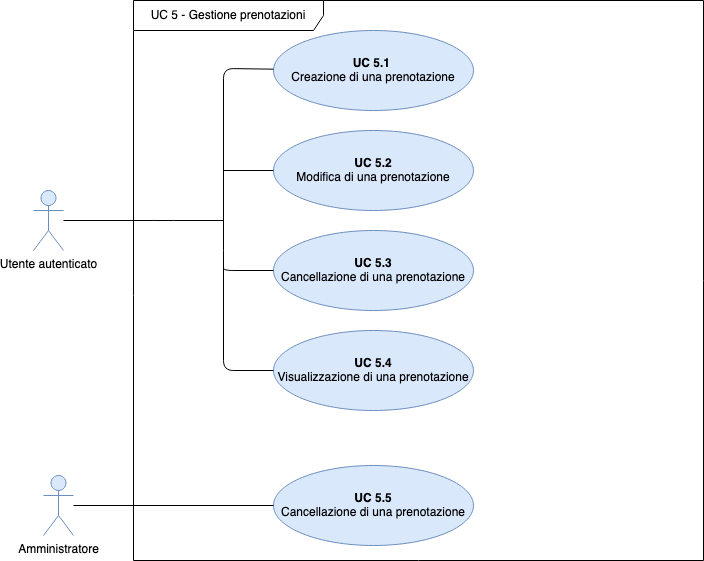
\includegraphics[scale=0.5]{src/CasiDUso/Immagini/UC5.png}
  \caption{UC  - Gestione di una prenotazione per un utente scelto}
\end{figure}

Il presente diagramma vuole riassumere la possibilità di gestione delle prenotazioni da parte di un amministratore registrato nell’applicazione.

\begin{itemize}
\item \textbf{Attori primari:} amministratore autenticato;
\item \textbf{Descrizione:} l'amministratore vuole gestire una prenotazione di un determinato utente scelto, a cui ha accesso a livello di permessi, con possibilità di creazione, modifica, eliminazione e visualizzazione;
\item \textbf{Precondizione:} l'amministratore è autenticato nell’applicazione e ha i permessi per eseguire le azioni di cui sopra;
\item \textbf{Postcondizione:} l'amministratore ha creato, modificato, eliminato o visualizzato una prenotazione;
\item \textbf{Scenario principale:} 
	\begin{itemize}
		\item l'amministratore è autenticato e naviga nell'apposita sezione riepilogativa delle prenotazioni dell'utente scelto;
		\item l'amministratore seleziona una prenotazione attiva dalla lista delle prenotazioni di un utente specifico o ne crea una nuova;
		\item l'amministratore crea, visualizza, modifica o rimuove una sua prenotazione;
		\item la prenotazione passa in stato di “pending” e, dopo una serie di controlli, viene confermata o eliminata.
	\end{itemize}
\end{itemize}

\subsubsection{UC 1.1 - Visualizzazione errore di prenotazione: prenotazione per determinata fascia oraria già esistente}
\begin{itemize}
\item \textbf{Attori primari:} utente autenticato;
\item \textbf{Precondizione:} l'utente sta cercando di prenotare una postazione in una data ed orario in cui la postazione risulta già prenotata da un altro utente;
\item \textbf{Postcondizione:} la prenotazione non viene approvata e l'utente riceve un messaggio di errore auto-esplicativo;
\item \textbf{Scenario principale:} l'utente visualizza un messaggio di errore in cui viene informato che la postazione risulta già occupata per la data e ora da lui scelti.
\end{itemize}

\subsubsection{UC 1.2 - Visualizzazione errore di prenotazione: postazione disabilitata da un amministratore}
\begin{itemize}
\item \textbf{Attori primari:} utente autenticato;
\item \textbf{Precondizione:} l'utente sta cercando di prenotare una postazione che risulta essere stata disabilitata da un amministratore;
\item \textbf{Postcondizione:} la prenotazione non viene approvata e l'utente riceve un messaggio di errore auto-esplicativo;
\item \textbf{Scenario principale:} l'utente visualizza un messaggio di errore in cui viene informato che la postazione risulta disabilitata e quindi non prenotabile.
\end{itemize}


\subsubsection{UC 2 - Modifica di una prenotazione per un utente scelto}

\begin{itemize}
\item \textbf{Attori primari:} amministratore autenticato;
\item \textbf{Descrizione:} l'amministratore vuole modificare una prenotazione già correttamente eseguita da un determinato utente, modificandone la data e/o orario;
\item \textbf{Precondizione:} l'amministratore è autenticato e naviga nell’apposita sezione di modifica di una prenotazione per un utente selezionato;
\item \textbf{Postcondizione:} l'amministratore modifica correttamente una prenotazione dell'utente selezionato con una nuova data/ora scelta;
\item \textbf{Scenario principale:} 
	\begin{itemize}
		\item il sistema elabora correttamente la richiesta, mandando in stato di “pending” la prenotazione;
		\item il sistema restituisce un errore per i seguenti motivi:
		\begin{itemize}
			\item la postazione è già stata prenotata per quella determinata fascia oraria[UC 1.1];
			\item la postazione è stata disabilitata da un amministratore di sistema[UC 1.2].	
		\end{itemize}
	\end{itemize}
\end{itemize}

\subsubsection{UC 3 - Cancellazione di una prenotazione}

\begin{itemize}
\item \textbf{Attori primari:} amministratore autenticato;
\item \textbf{Descrizione:} l'amministratore vuole cancellare una prenotazione per una certa data od orario effettuata in precedenza da un determinato utente;
\item \textbf{Precondizione:} l'amministratore è autenticato e naviga nell’apposita sezione di cancellazione di una prenotazione per un utente selezionato;
\item \textbf{Postcondizione:} l'amministratore cancella correttamente la prenotazione di un utente per la data/ora scelta;
\item \textbf{Scenario principale:} 
	\begin{itemize}
		\item il sistema elabora correttamente la richiesta;
		\item il sistema restituisce un errore per i seguenti motivi:
		\begin{itemize}
			\item non è possibile cancellare una prenotazione per un orario passato[UC 3.1].
		\end{itemize}
	\end{itemize}
\end{itemize}

\subsubsection{UC 3.1 - Visualizzazione errore di cancellazione: tentativo di cancellazione di una prenotazione per un orario passato}
\begin{itemize}
\item \textbf{Attori primari:} utente autenticato;
\item \textbf{Precondizione:} l'utente sta cercando di cancellare una prenotazione già usufruita in un orario passato;
\item \textbf{Postcondizione:} la cancellazione non viene approvata e l'utente riceve un messaggio di errore auto-esplicativo;
\item \textbf{Scenario principale:} l'utente visualizza un messaggio di errore in cui viene informato che non è possibile cancellare una prenotazione per un orario antecedente a quello attuale.
\end{itemize}

\subsubsection{UC 4 - Visualizzazione di una prenotazione}

\begin{itemize}
\item \textbf{Attori primari:} amministratore autenticato;
\item \textbf{Descrizione:} l'amministratore vuole visualizzare le prenotazioni attive nel sistema di un determinato utente;
\item \textbf{Precondizione:} l'amministratore è autenticato e naviga nell’apposita sezione di visualizzazione delle prenotazioni di un utente selezionato;
\item \textbf{Postcondizione:} l'amministratore visualizza correttamente le prenotazioni attive di un utente selezionato;
\item \textbf{Scenario principale:} 
	\begin{itemize}
		\item il sistema elabora correttamente la richiesta;
		\item il sistema restituisce un errore per i seguenti motivi:
		\begin{itemize}
			\item l'utente selezionato non ha alcuna prenotazione attiva[UC4.1].
		\end{itemize}
	\end{itemize}
\end{itemize}

\subsubsection{UC 4.1 - Visualizzazione errore di prenotazione attiva: l'utente non ha alcuna prenotazione attiva}
\begin{itemize}
\item \textbf{Attori primari:} utente autenticato;
\item \textbf{Precondizione:} l'utente sta cercando di visualizzare la lista delle sue prenotazioni, non avendone però alcuna attiva;
\item \textbf{Postcondizione:} la visualizzazione non viene eseguita e l'utente riceve un messaggio di errore auto-esplicativo;
\item \textbf{Scenario principale:} l'utente visualizza un messaggio di errore in cui viene informato che non ha alcuna prenotazione attiva.
\end{itemize}

\subsubsection{UC 5 - Disabilitazione di una postazione}

\begin{itemize}
\item \textbf{Attori primari:} amministratore autenticato;
\item \textbf{Descrizione:} l’amministratore vuole impedire la prenotazione di una specifica postazione da parte di utenti autenticati;
\item \textbf{Precondizione:} l’amministratore è autenticato e naviga nell’apposita sezione di blocco prenotazione di una postazione;
\item \textbf{Postcondizione:} l’amministratore blocca correttamente la possibilità di prenotare una postazione per qualsiasi utente autenticato;
\item \textbf{Scenario principale:} 
	\begin{itemize}
		\item il sistema elabora correttamente la richiesta;
		\end{itemize}
\end{itemize}
